\section{Results}\label{sec:results}

\subsection{Grid and feasible set}
Table~\ref{tab:grid} gives the grid swept for each layout and the number of feasible designs. In total 1053 designs were attempted and 969 were feasible. After the first sweep, we added two refinement grids around the best layout~3 and layout~6 designs. Layout~2 was swept most finely because it sets the calibration. The other layouts were swept at $\Tt = \SI{500}{\celsius}$ only, because the layout~2 sweep showed that efficiency always rises with $\Tt$ (best efficiency 33.3\% at \SI{500}{\celsius}, 32.7\% at \SI{475}{\celsius}, 32.0\% at \SI{451}{\celsius}).

\begin{table}[h]\centering\small
\begin{tabularx}{\textwidth}{@{}c X c c l@{}}
\toprule
Layout & Grid (pressures in MPa, $\Tin$ in \si{\celsius}) & Attempted & Feasible & Rejected\\
\midrule
1 & $\Ph$ 16--20 (step 2); $\Pl$ 7.7, 8.7; $\Tin$ 32, 36, 40 & 18 & 9 & 9 solver error\\
2 & $\Ph$ 14--20 (step 1); $\Pl$ 7.7--9.7 (step 0.5); $\Tin$ 32--40 (step 2); $\Tt$ 500, 475, 451 & 525 & 512 & 13 pinch\\
3 & $\Ph$ 16--20 (step 2); $\Pl$ 7.7, 8.2; $\Tin$ 32, 36, 40; $x$ 0.15--0.40 (step 0.05). Refinement at 20 / 7.7 MPa: $\Tin$ 32, 33, 34; $x$ 0.30--0.40 (step 0.01) & 138 & 136 & 2 pinch\\
4 & as layout 3 without $x$; $\Pm$ 10, 12, 14 & 54 & 53 & 1 cross\\
5 & $\Ph$ 18, 20; $\Pl$ 7.7, 8.2; $\Tin$ 32, 36, 40; $x$ 0.20--0.35; $\Pm$ 10, 12, 14 & 144 & 91 & 44 pinch, 9 cross\\
6 & $\Ph$ 18, 20; $\Pm$ 7.7, 8.2, 8.7; $\Pe$ 5.5, 6.5, 7.5; $\Tin$ 32, 36, 40; $x$ 0.2, 0.3, 0.4. Refinement at 20 / 7.7 MPa: $\Pe$ 4.5, 5.5; $\Tin$ 32, 36; $x$ 0.35, 0.45, 0.50 & 174 & 168 & 6 pinch\\
\bottomrule
\end{tabularx}
\caption{Grid and feasible set per layout. ``Pinch'' means a recuperator temperature difference below \SI{5}{K}. ``Cross'' is a temperature cross, a recuperator pinch below zero.}\label{tab:grid}
\end{table}

\paragraph{Layout 1 limitation.} Nine of the 18 layout~1 designs did not solve. Without a recuperator the cooler receives turbine exhaust at about \SI{400}{\celsius}, and the search for the cooling-water flow reaches the boiling point of water at the solver's coolant pressure of \SI{6}{bar} (\SI{159}{\celsius}). This is a limit of the cooler model, not of the cycle. The nine designs that solved have efficiencies of 10\% to 15\%, far below every other layout, so the missing points cannot change any conclusion.

\code{\path{grids.py}, \path{core/make_inputs.py}, \path{core/solve_points.py}, \path{data/inputs.csv}, \path{data/infeasible.csv}}

\subsection{Calibration}
The most efficient feasible layout~2 design is $\Ph = \SI{20}{MPa}$, $\Pl = \SI{7.7}{MPa}$, $\Tin = \SI{34}{\celsius}$, $\Tt = \SI{500}{\celsius}$, with $\eta = 33.3\%$. Its recuperator has $UA = \SI{1866}{kW/K}$ (\SI{4.66}{t}) and its cooler $UA = \SI{6511}{kW/K}$ (\SI{16.28}{t}), so
\[ M_0 = 60 - 4.66 - 16.28 = \SI{39.06}{t}. \]
The best inlet temperature is \SI{34}{\celsius} and not the \SI{32}{\celsius} limit. At \SI{32}{\celsius} the compressor work is lower, but the recuperator recovers less heat at fixed effectiveness, and the second effect is larger here. This design, called the recuperated reference from here on, is the baseline for every comparison in the rest of the report.

\code{\path{core/calibrate.py}}

\subsection{Efficiency trends}
\begin{figure}[h]\centering
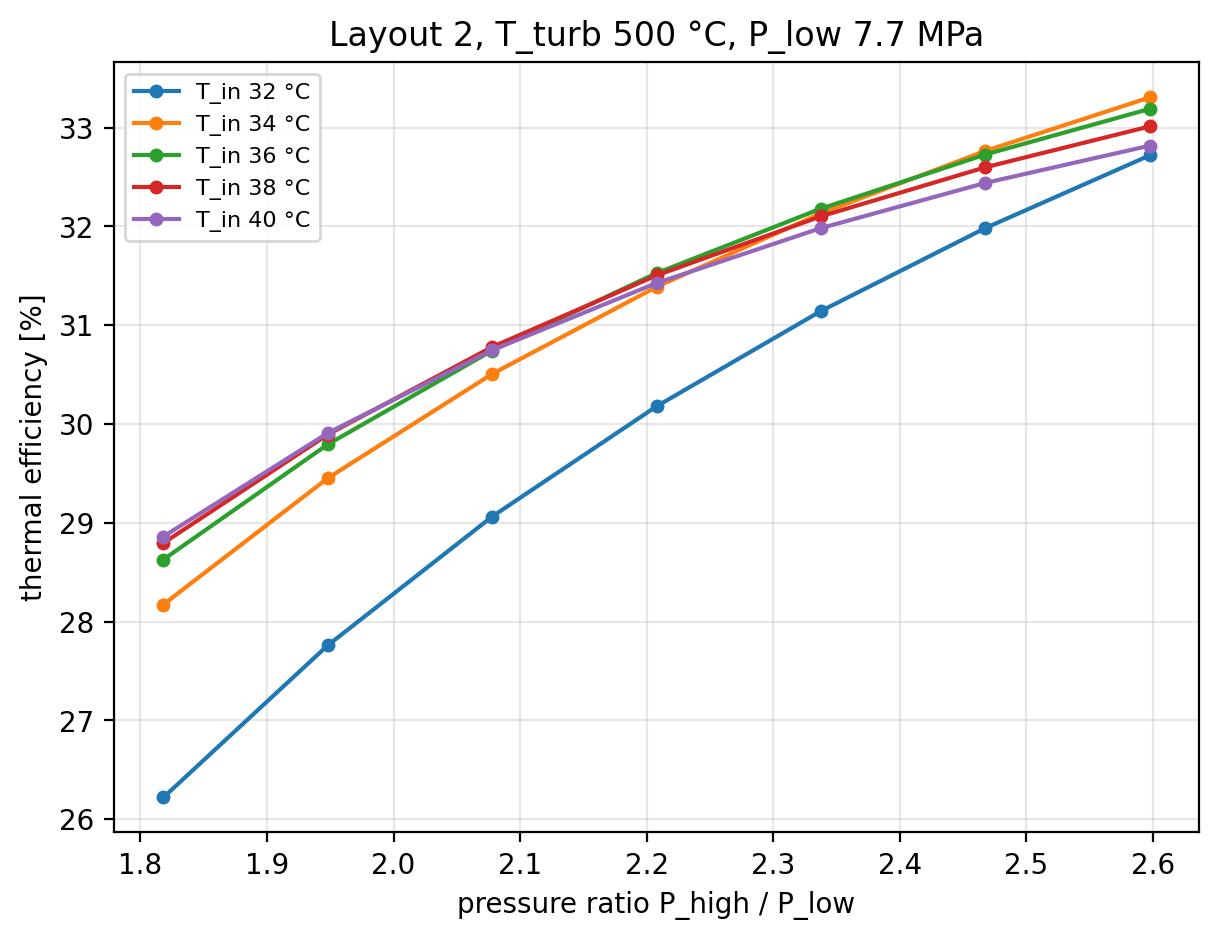
\includegraphics[width=0.49\textwidth]{figs/eta_vs_pressure_ratio.png}\hfill
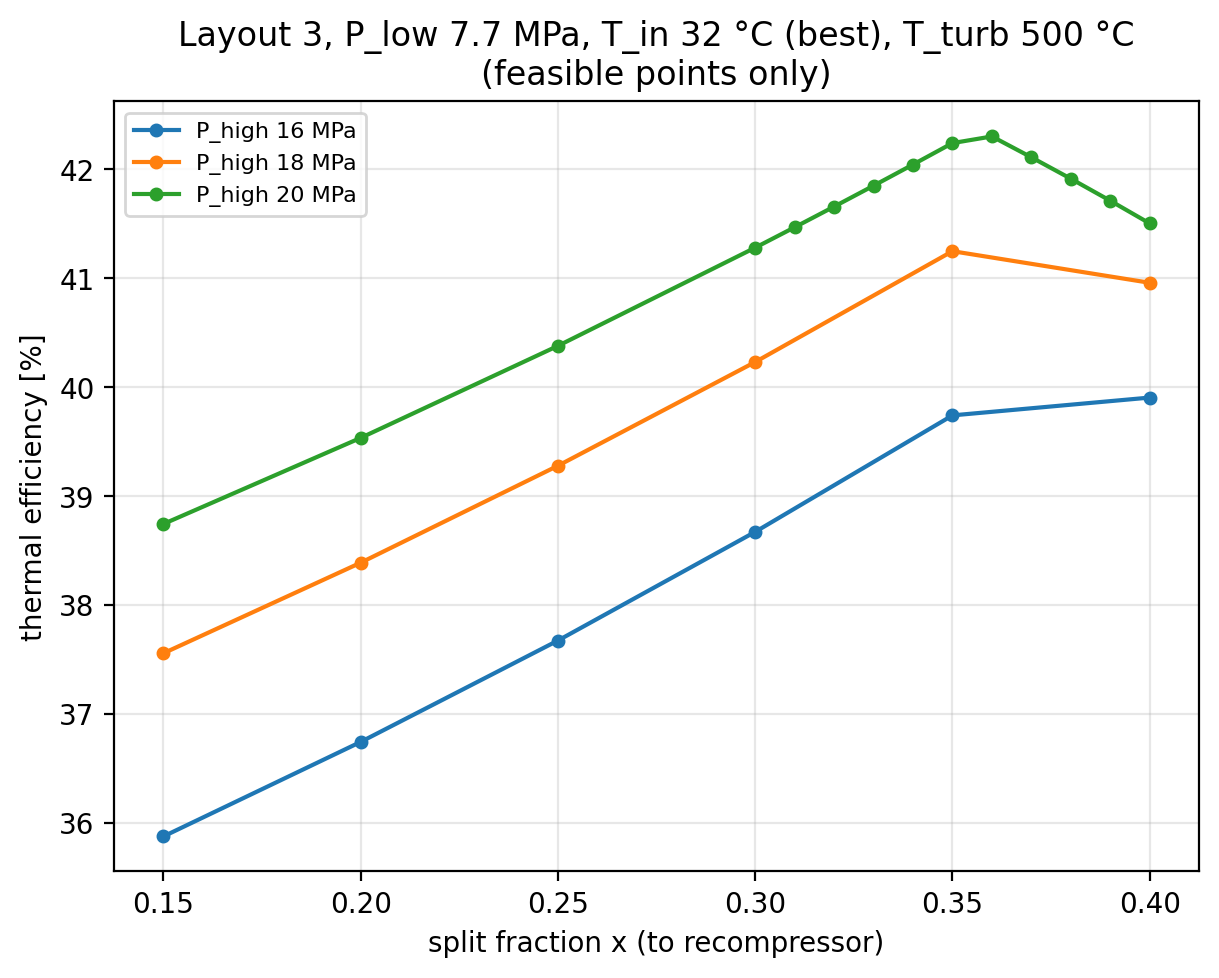
\includegraphics[width=0.49\textwidth]{figs/eta_vs_split.png}
\caption{Efficiency against pressure ratio (left) and against split fraction (right).}\label{fig:trends}
\end{figure}
In every layout the efficiency rises with $\Ph$ up to the \SI{20}{MPa} limit, so the best pressure ratio is the largest one allowed, $20/7.7 = 2.6$. For layout~2 the best efficiency at \SI{500}{\celsius} rises from 28.9\% at \SI{14}{MPa} to 33.3\% at \SI{20}{MPa}. For recompression at \SI{20}{MPa}, \SI{7.7}{MPa} and \SI{32}{\celsius}, efficiency rises with split fraction from 38.7\% at $x = 0.15$ to a maximum of 42.3\% at $x = 0.36$, then falls to 41.5\% at $x = 0.40$. The optimum split for efficiency is 0.36, where the heat capacities of the two streams in the low-temperature recuperator are balanced. Beyond it, the recompressor work grows faster than the heat recovery. The mass also falls beyond 0.36 (from \SI{78.2}{t} to \SI{74.6}{t} at $x = 0.40$), because the temperature difference in the low-temperature recuperator opens from \SI{10}{K} to \SI{18}{K} and it needs less conductance. This is why the rankings that include mass prefer splits above the efficiency optimum.

\code{\path{core/plots.py}, \path{data/results_raw.csv}}

\subsection{Best design of each layout}
\begin{table}[h]\centering\small
\setlength{\tabcolsep}{4pt}\begin{tabular}{@{}clcccccc@{}}
\toprule
Layout & Best design (by payout) & $\eta$ & $\eta_\mathrm{II}$ & $UA$ & Mass & Payout & Sp. power\\
 & & (\%) & (\%) & (kW/K) & (t) & (M\$) & (MWe/t)\\
\midrule
1 & 20 / 7.7 MPa, \SI{32}{\celsius} & 14.8 & 24.5 & 3851 & 48.7 & 60.4 & 0.30\\
2 & 20 / 7.7 MPa, \SI{34}{\celsius} & 33.3 & 55.3 & 8376 & 60.0 & 148.2 & 0.56\\
3 & 20 / 7.7 MPa, \SI{32}{\celsius}, $x = 0.36$ & 42.3 & 69.9 & 15074 & 78.2 & 187.7 & 0.54\\
4 & 20 / 8.2 MPa, \SI{32}{\celsius}, $\Pm = 14$ & 34.1 & 56.3 & 13992 & 75.5 & 148.1 & 0.45\\
5 & 20 / 7.7 MPa, \SI{32}{\celsius}, $\Pm = 10$, $x = 0.35$ & 42.5 & 70.1 & 17763 & 86.5 & 186.4 & 0.49\\
6 & 20 / 7.7 MPa, $\Pe = 5.5$, \SI{32}{\celsius}, $x = 0.45$ & 41.6 & 68.7 & 14110 & 77.3 & 184.5 & 0.54\\
\bottomrule
\end{tabular}
\caption{Best design of each layout by 10-year payout. All at $\Tt = \SI{500}{\celsius}$. Pressures are written as compressor outlet / main compressor inlet ($\Ph$ / $\Pl$). In layout~6 the main compressor inlet is at $\Pm$, and the turbine exhausts to the lower pressure $\Pe$, which is the pre-compressor inlet.}\label{tab:best}
\end{table}

Compared with the expectations of Section~\ref{sec:layouts}:
\begin{itemize}
  \item \textbf{Recuperation is essential.} Layout~1 reaches only 14.8\%. Recuperation more than doubles this for \SI{11}{t} more hardware.
  \item \textbf{Recompression gives the large gain.} Layout~3 adds 9.0 points of efficiency over layout~2. It needs almost twice the conductance, because the two recuperators work at smaller temperature differences.
  \item \textbf{Intercooling does not pay.} Layout~4 gains 0.8 points over layout~2 for \SI{15.5}{t} more mass, and its payout is no better. Layout~5 gains 0.2 points over layout~3 for \SI{8.2}{t} more. \scotwo{} compression near the critical point already takes little work, so there is little left to save.
  \item \textbf{Partial cooling is close to recompression.} Layout~6 reaches 41.6\% at slightly lower mass than the best layout~3 design, but with one more compressor and one more cooler, and its payout is \$3.3M lower. Its pre-compressor inlet is below the \SI{7.7}{MPa} limit in every design (Section~\ref{sec:objective}).
\end{itemize}

\code{\path{core/summary.py}, \path{out/summary.md}}

\subsection{Pareto front, knee and TOPSIS}
\begin{figure}[h]\centering
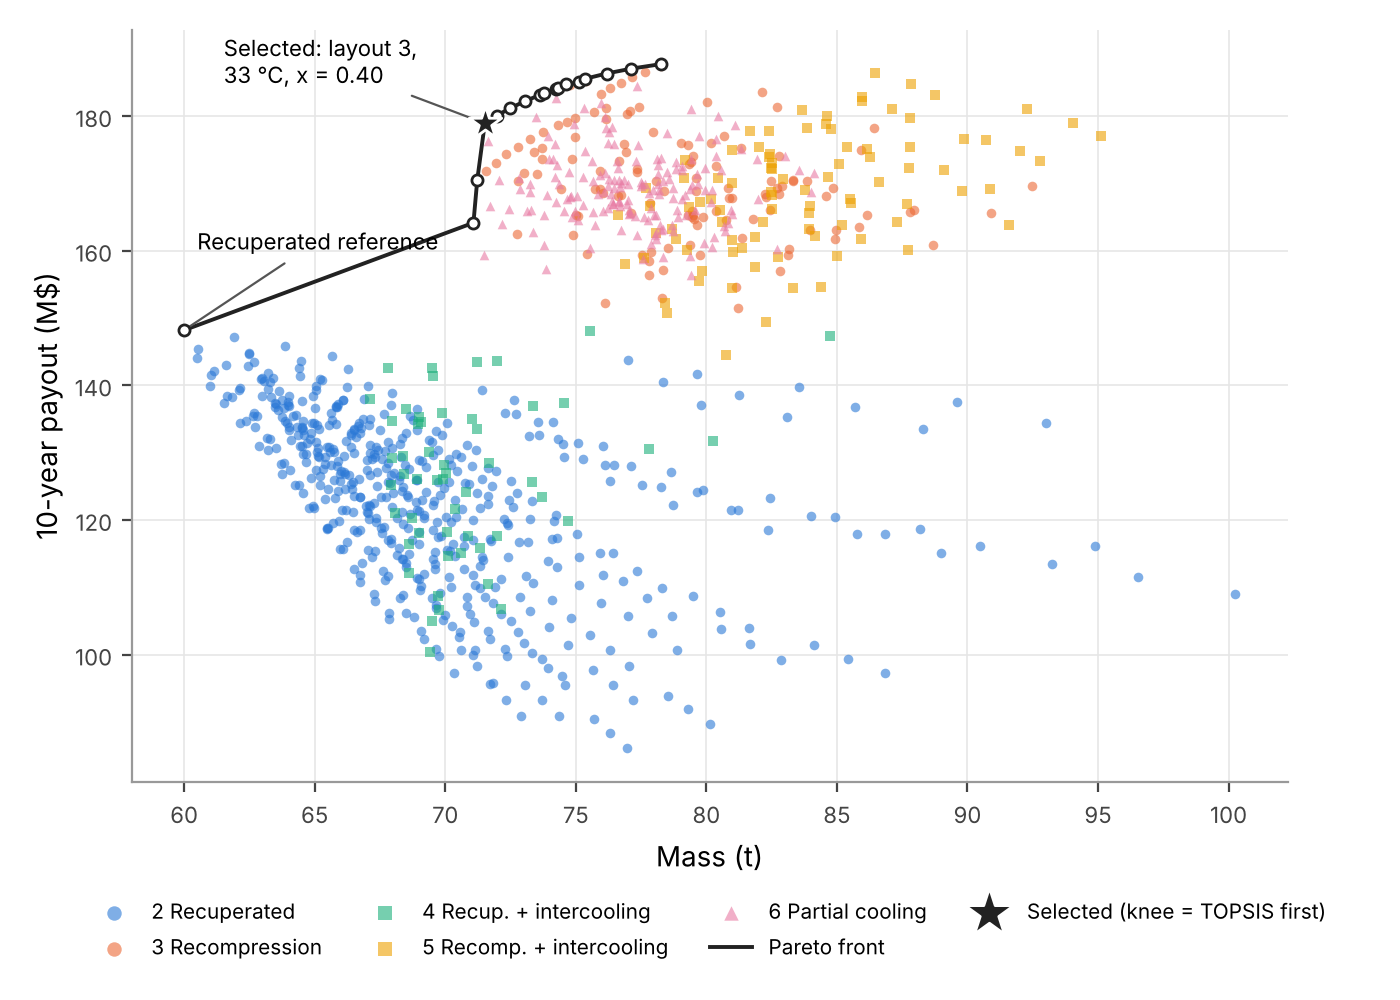
\includegraphics[width=0.82\textwidth]{figs/pareto_noL1.png}
\caption{Ten-year payout against mass for layouts 2 to 6, with the Pareto front and the selected design.}\label{fig:pareto}
\end{figure}
\begin{figure}[h]\centering
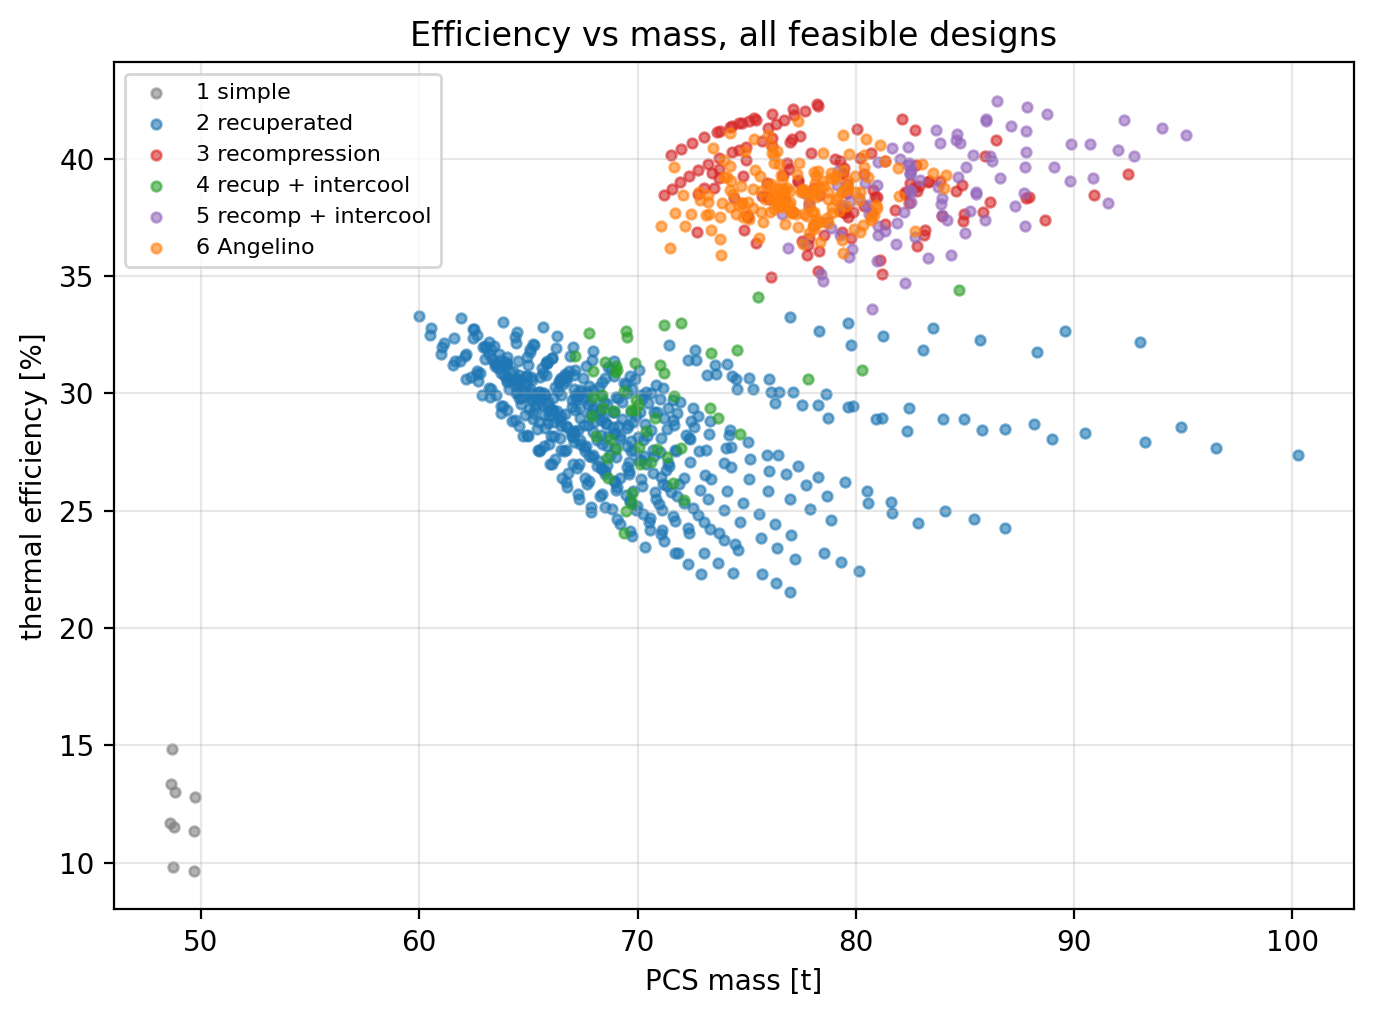
\includegraphics[width=0.6\textwidth]{figs/eta_vs_mass.png}
\caption{Efficiency against mass, all layouts.}\label{fig:etamass}
\end{figure}
With the simple cycle left out (Section~\ref{sec:objective}), 17 designs lie on the Pareto front of payout against mass (Figure~\ref{fig:pareto}). They fall into two groups. The first is the recuperated reference on its own, at \SI{60}{t} and \$148M. The second is sixteen designs between \SI{71}{t} and \SI{78}{t}, with payouts from \$164M to \$188M. Fifteen of these are recompression designs at \SI{20}{MPa} and \SI{7.7}{MPa}, with $\Tin$ from \SI{32}{\celsius} to \SI{34}{\celsius} and $x$ from 0.30 to 0.40; the sixteenth is a partial cooling design. No intercooled design (layout~4 or~5) reaches the front: each is beaten by a design that is both lighter and earns more.

\paragraph{Knee.} The knee is the recompression design at $\Tin = \SI{33}{\celsius}$ and $x = 0.40$ (\SI{71.5}{t}, \$178.9M), where the front turns. Towards lighter designs the payout falls steeply, by \$30.7M over the \SI{11.5}{t} down to the recuperated reference. Towards heavier designs each extra tonne adds only about \$1.3M, up to \$187.7M at \SI{78.2}{t}.

\paragraph{TOPSIS.} With equal weights, TOPSIS ranks the same design first (Table~\ref{tab:topsis}), so the two methods agree; this also holds with the simple cycle included. The leading scores are close, and the first four designs are the same recompression cycle at \SI{33}{\celsius} with $x$ from 0.37 to 0.40. The ranking therefore points to a region, $\Tin \approx \SI{33}{\celsius}$ with $x$ between 0.37 and 0.40, rather than to a single point. The recuperated reference ranks 130th: it is the lightest design on the front, but its payout is far below the rest.

\begin{table}[h]\centering\small
\begin{tabular}{@{}cllcccc@{}}
\toprule
Rank & Layout & Design & $\eta$ (\%) & Mass (t) & Payout (M\$) & Score\\
\midrule
1 & 3 & 20 / 7.7 MPa, \SI{33}{\celsius}, $x = 0.40$ & 40.2 & 71.5 & 178.9 & 0.818\\
2 & 3 & 20 / 7.7 MPa, \SI{33}{\celsius}, $x = 0.39$ & 40.4 & 72.0 & 180.1 & 0.816\\
3 & 3 & 20 / 7.7 MPa, \SI{33}{\celsius}, $x = 0.38$ & 40.7 & 72.5 & 181.2 & 0.813\\
4 & 3 & 20 / 7.7 MPa, \SI{33}{\celsius}, $x = 0.37$ & 40.9 & 73.0 & 182.2 & 0.808\\
5 & 6 & 20 / 7.7 MPa, $\Pe = 4.5$, \SI{32}{\celsius}, $x = 0.35$ & 39.6 & 71.6 & 176.3 & 0.806\\
\bottomrule
\end{tabular}
\caption{Top five designs by TOPSIS, layouts 2 to 6, weights 0.5 on payout and 0.5 on mass. Pressures are written as compressor outlet / main compressor inlet ($\Ph$ / $\Pl$). In layout~6 the main compressor inlet is at $\Pm$, and the turbine exhausts to the lower pressure $\Pe$, which is the pre-compressor inlet.}\label{tab:topsis}
\end{table}

\code{\path{helpers/ranking.py}, \path{data/results_econ.csv}}

\subsection{Selected design}
The selected design is the recompression cycle at $\Ph = \SI{20}{MPa}$, $\Pl = \SI{7.7}{MPa}$, $\Tin = \SI{33}{\celsius}$, $\Tt = \SI{500}{\celsius}$ and $x = 0.40$. It is the knee of the Pareto front and first by TOPSIS. Table~\ref{tab:selected} gives its performance and Table~\ref{tab:selstates} its states, re-solved with 100 cooler slices.

\begin{table}[h]\centering\small
\begin{tabular}{@{}lr@{\qquad}lr@{}}
\toprule
Thermal efficiency & 40.2\% & Net power & \SI{40.2}{MWe}\\
Carnot efficiency & 60.4\% & Second-law efficiency & 66.5\%\\
High-temperature recuperator $UA$ & \SI{3664}{kW/K} & Its pinch & \SI{19.1}{K}\\
Low-temperature recuperator $UA$ & \SI{2759}{kW/K} & Its pinch & \SI{18.6}{K}\\
Cooler $UA$ & \SI{5960}{kW/K} & Its pinch & \SI{5.0}{K}\\
Mass & \SI{71.5}{t} & Volume & \SI{143}{m^3}\\
Hardware cost & \$17.9M & Electricity revenue & \$19.7M per year\\
10-year payout & \$178.9M & Specific power & \SI{0.562}{MWe/t}\\
\cotwo{} flow & \SI{553}{kg/s} & Cooling-water flow & \SI{638}{kg/s}\\
\bottomrule
\end{tabular}
\caption{Selected design.}\label{tab:selected}
\end{table}

\begin{table}[h]\centering\small
\begin{tabular}{@{}lccccc@{}}
\toprule
State & $P$ (MPa) & $T$ (\si{\celsius}) & $h$ (kJ/kg) & $s$ (kJ/kg\,K) & Flow fraction\\
\midrule
Main compressor inlet & 7.7 & 33.0 & 345.8 & 1.476 & 0.6\\
Main compressor outlet & 20 & 78.2 & 371.5 & 1.484 & 0.6\\
Low-temperature recuperator, cold outlet & 20 & 200.7 & 598.8 & 2.049 & 0.6\\
Recompressor outlet & 20 & 199.3 & 596.8 & 2.044 & 0.4\\
After mixing & 20 & 200.1 & 598.0 & 2.047 & 1\\
High-temperature recuperator, cold outlet & 20 & 352.6 & 792.4 & 2.404 & 1\\
Turbine inlet & 20 & 500.0 & 973.3 & 2.664 & 1\\
Turbine outlet & 7.7 & 390.6 & 857.0 & 2.683 & 1\\
High-temperature recuperator, hot outlet & 7.7 & 219.3 & 662.5 & 2.345 & 1\\
Low-temperature recuperator, hot outlet & 7.7 & 103.1 & 526.2 & 2.028 & 1\\
\bottomrule
\end{tabular}
\caption{States of the selected design.}\label{tab:selstates}
\end{table}

\begin{figure}[h]\centering
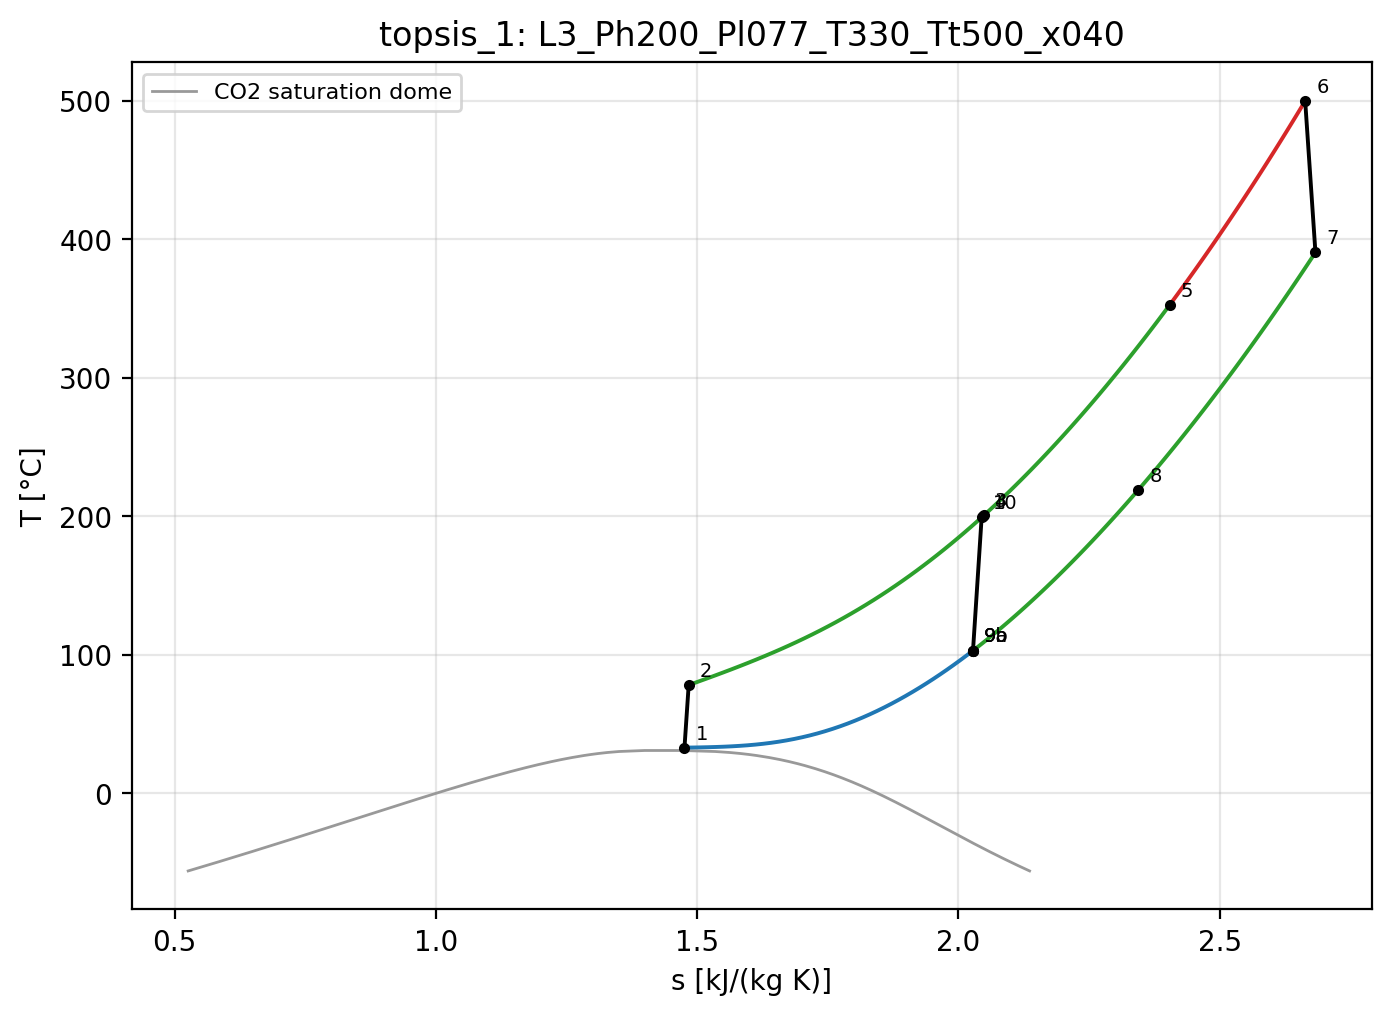
\includegraphics[width=0.49\textwidth]{figs/ts_selected.png}\hfill
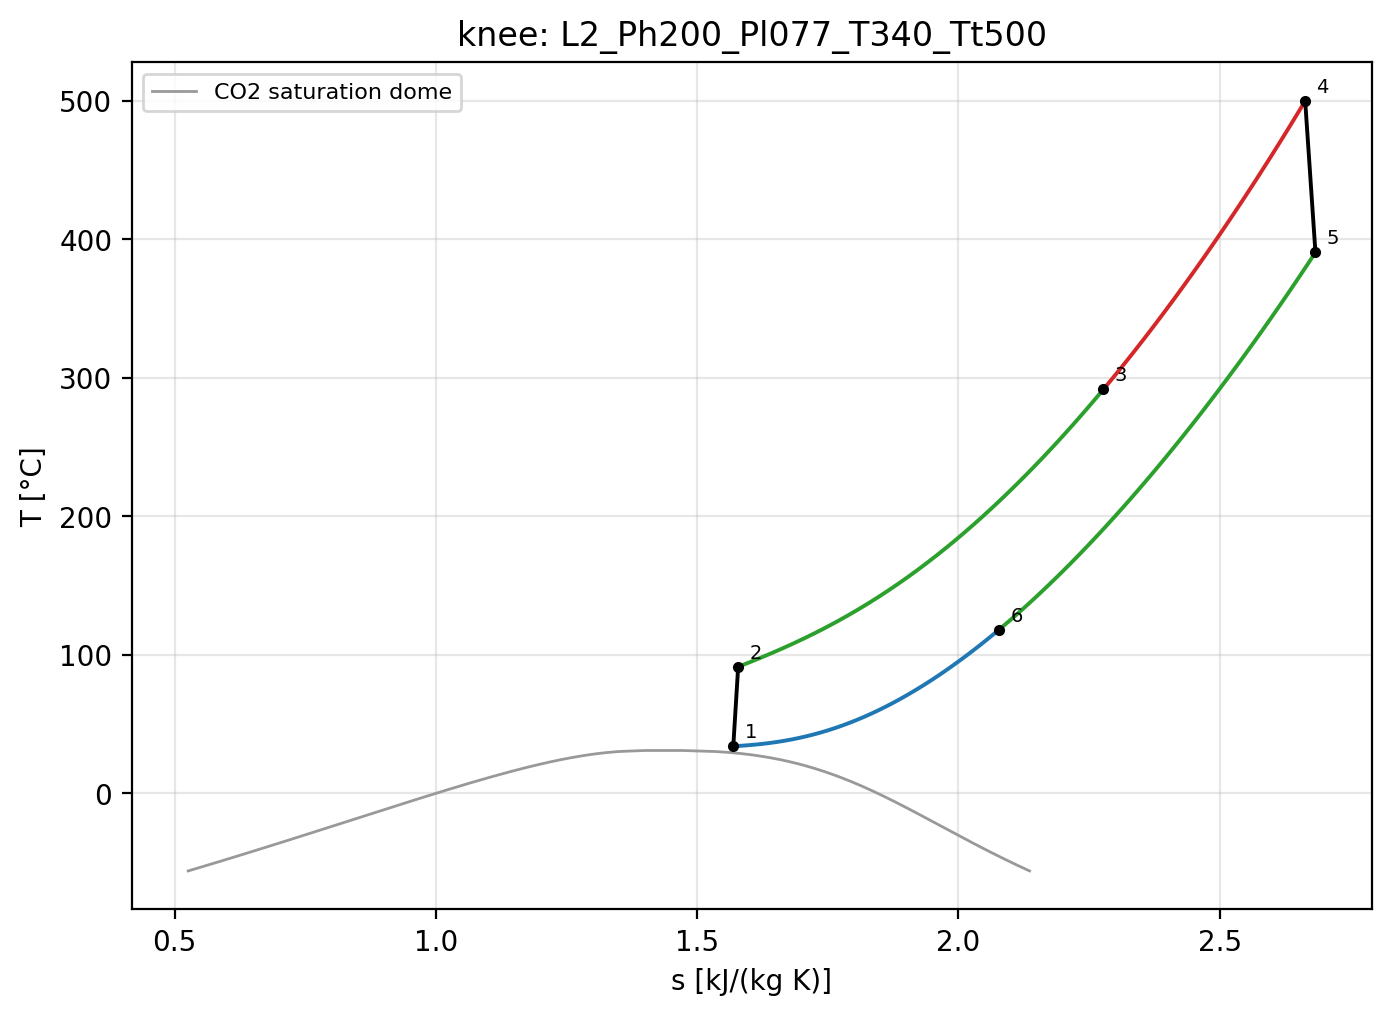
\includegraphics[width=0.49\textwidth]{figs/ts_baseline.png}
\caption{$T$--$s$ diagrams of the selected recompression design (left) and the layout~2 reference (right).}\label{fig:ts}
\end{figure}

The compressor inlet is \SI{2.0}{K} and \SI{0.32}{MPa} above the critical point (\SI{30.98}{\celsius}, \SI{7.377}{MPa}). The turbine inlet pressure and temperature and the compressor inlet pressure are at their limits. The inlet temperature and the split fraction are not. Raising the inlet from \SI{32}{\celsius} to \SI{33}{\celsius} costs 1.3 points of efficiency at the same split, but the cooler then rejects heat at a larger temperature difference, the cooling-water flow halves (\SI{638}{kg/s} against \SI{1282}{kg/s}), and the exchangers are \SI{3.1}{t} lighter.

\code{\path{core/export_states.py}, \path{data/shortlist.csv}, \path{data/states.csv}, \path{out/Top_N_topsis/}}

\subsection{What is given up}
\begin{itemize}
  \item \textbf{Against the highest-payout design} (layout~3, \SI{32}{\celsius}, $x = 0.36$; 42.3\%, \SI{78.2}{t}, \$187.7M): the selected design gives up 2.1 points of efficiency and \$8.8M of payout (4.7\%), and saves \SI{6.7}{t} (8.6\%).
  \item \textbf{Against the most efficient design} (layout~5; 42.5\%, \SI{86.5}{t}, \$186.4M): it gives up 2.3 points of efficiency and \$7.5M of payout, and is \SI{15.0}{t} lighter with one fewer compressor and one fewer cooler.
  \item \textbf{Against the layout~2 reference} (33.3\%, \SI{60}{t}, \$148.2M): it is \SI{11.5}{t} heavier, which costs \$2.9M, and its extra output is worth \$3.4M per year. The incremental payback is about 10 months (Table~\ref{tab:increment}), and the ten-year payout is \$30.7M higher.
  \item \textbf{Against the simple cycle} (layout~1, \SI{48.7}{t}, \$60.4M, outside the ranking): it is \SI{23}{t} heavier and earns about three times the payout.
\end{itemize}

\paragraph{Comparison with the baseline, step by step.} Table~\ref{tab:increment} repeats the given worked comparison with the computed values of the recuperated reference and the selected design. All values are per year of operation at \SI{7000}{h}. The payback in the last row is the incremental payback of Section~\ref{sec:objective}: it compares the added hardware with the added output only.

\begin{table}[h]\centering\small
\begin{tabular}{@{}r l l l@{}}
\toprule
 & Quantity & Calculation & Value\\
\midrule
1 & Reference net power & $0.3331 \times 100$ & \SI{33.31}{MWe}\\
2 & Reference heat per MWe & $100/33.31$ & \SI{3.00}{MWth/MWe}\\
3 & Candidate net power & $0.4017 \times 100$ & \SI{40.17}{MWe} (\SI{2.49}{MWth/MWe})\\
4 & Extra output & $40.17 - 33.31$ & \SI{6.86}{MWe}\\
5 & Extra annual energy & $6.86 \times 7000$ & \SI{48030}{MWh}\\
6 & Extra annual value & $48030 \times 70$ & \$3.36M per year\\
7 & Added mass & $71.52 - 60.00$ & \SI{11.52}{t}\\
8 & Added hardware cost & $11520 \times 250$ & \$2.88M\\
9 & Compactness & $33.31/60.00$ against $40.17/71.52$ & 0.555 against \SI{0.562}{MWe/t}\\
10 & Second-law efficiency & $\eta/\eta_\mathrm{Carnot}$ & 0.553 against 0.665\\
11 & Incremental payback & $2.88/3.36$ & 0.86 years (about 10 months)\\
\bottomrule
\end{tabular}
\caption{Selected design against the recuperated reference, following the given worked comparison.}\label{tab:increment}
\end{table}

The selected design is more compact than the reference in MWe per tonne as well as more efficient: the extra exchanger mass is more than matched by the extra output. Under the omissions listed in Section~\ref{sec:limits}, the added hardware is recovered within the first year of operation.

\code{\path{data/results_econ.csv}, \path{out/summary.md}}

\subsection{Sensitivity}
We test whether the selection survives changes in two things: the lifetime $N$ and the grid spacing.

\paragraph{Lifetime $N$: the selection holds.} The payout weighs efficiency against hardware, $\Pi_N = N\,\eta\,\dot Q_\mathrm{th}\,t_\mathrm{op}\,c_e - c_m\,m$. A larger $N$ gives efficiency more weight and favours heavier, more efficient designs; a smaller $N$ favours light ones. We repeated the ranking for $N$ = 5, 10 and 20 years (Table~\ref{tab:life}). The knee and TOPSIS pick the same design at all three, and the highest-payout design does not change either. The recommendation therefore does not hinge on the choice of ten years.

\begin{table}[h]\centering\small
\setlength{\tabcolsep}{4pt}\begin{tabular}{@{}clll@{}}
\toprule
$N$ (years) & Knee & TOPSIS first & Highest payout\\
\midrule
5 & L3, \SI{33}{\celsius}, $x = 0.40$ (\$80.5M) & L3, \SI{33}{\celsius}, $x = 0.40$ (\$80.5M) & L3, \SI{32}{\celsius}, $x = 0.36$ (\$84.1M)\\
10 & L3, \SI{33}{\celsius}, $x = 0.40$ (\$178.9M) & L3, \SI{33}{\celsius}, $x = 0.40$ (\$178.9M) & L3, \SI{32}{\celsius}, $x = 0.36$ (\$187.7M)\\
20 & L3, \SI{33}{\celsius}, $x = 0.40$ (\$375.8M) & L3, \SI{33}{\celsius}, $x = 0.40$ (\$375.8M) & L3, \SI{32}{\celsius}, $x = 0.36$ (\$395.0M)\\
\bottomrule
\end{tabular}
\caption{Sensitivity to the lifetime $N$, layouts 2 to 6. L3 is layout 3.}\label{tab:life}
\end{table}

\paragraph{Grid spacing: partly stable.} In the first sweep, with inlet temperatures of 32, 36 and \SI{40}{\celsius} and a split step of 0.05, TOPSIS picked layout~3 at \SI{20}{MPa} and \SI{7.7}{MPa}, \SI{32}{\celsius} and $x = 0.40$. After the refinement, with inlet temperatures of 32, 33 and \SI{34}{\celsius} and a split step of 0.01, it picked the same layout and pressures at \SI{33}{\celsius} and $x = 0.40$. The layout and pressures never moved, so they are firm. The inlet temperature moved by one grid step, so it is known only to about the grid spacing.

\code{\path{core/summary.py}}

\subsection{Cautions on the selected design}
\paragraph{The optimum split may lie just past the grid.} The refined split range ends at 0.40, and the TOPSIS score is still rising there (Table~\ref{tab:splitedge}). When the best point sits on the boundary of the search and the trend is still upward, the true optimum is probably a little beyond it, perhaps at 0.41 to 0.43. The gains shrink with each step, so it is unlikely to be far. This is why we state the split only to about 0.02 and the inlet temperature to about \SI{1}{K}, the refined grid step.

\begin{table}[h]\centering\small
\begin{tabular}{@{}lcccccc@{}}
\toprule
Split fraction $x$ & 0.35 & 0.36 & 0.37 & 0.38 & 0.39 & 0.40\\
\midrule
TOPSIS score & 0.796 & 0.803 & 0.808 & 0.813 & 0.816 & 0.818\\
\bottomrule
\end{tabular}
\caption{TOPSIS score against split fraction for layout~3 at \SI{20}{MPa}, \SI{7.7}{MPa} and \SI{33}{\celsius}.}\label{tab:splitedge}
\end{table}

\paragraph{The inlet sits at the steepest part of the \cotwo{} property curve.} The critical point of \cotwo{} is \SI{30.98}{\celsius} and \SI{7.38}{MPa}. At \SI{7.7}{MPa}, just above the critical pressure, \cotwo{} changes from liquid-like to gas-like over a narrow band of temperature, and the selected inlet lies inside that band (Table~\ref{tab:inletprops}). At \SI{33}{\celsius} the specific heat is almost exactly at its peak. A drift of \SI{1}{K} either way changes the density by more than 20\%, which changes the work and flow of the compressor substantially. In a real plant the inlet temperature wanders with the cooling-water temperature, the load and the control system. This study computes one steady design point and does not examine how the cycle behaves when the inlet drifts (off-design or transient operation). The computed efficiency therefore assumes that the inlet is held tightly at \SI{33}{\celsius}, which we have not shown to be achievable.

\begin{table}[h]\centering\small
\begin{tabular}{@{}lcccc@{}}
\toprule
Inlet temperature (\si{\celsius}) & 32 & \textbf{33} & 34 & 36\\
\midrule
Density (\si{kg/m^3}) & 602 & \textbf{431} & 338 & 289\\
$c_p$ (\si{kJ/kg.K}) & 15.1 & \textbf{65.5} & 14.9 & 6.8\\
\bottomrule
\end{tabular}
\caption{\cotwo{} properties at \SI{7.7}{MPa} near the selected compressor inlet temperature (CoolProp).}\label{tab:inletprops}
\end{table}

\section{Recommendation}
The recommended cycle is the \textbf{recompression cycle (layout 3)} at \SI{20}{MPa} turbine inlet pressure, \SI{7.7}{MPa} and \SI{33}{\celsius} compressor inlet, \SI{500}{\celsius} turbine inlet and a split fraction of 0.40. It delivers \SI{40.2}{MWe} at 40.2\% efficiency, has a mass of \SI{71.5}{t}, and returns \$178.9M over ten years.

The reasons are:
\begin{enumerate}
  \item It is the knee of the Pareto front and is ranked first by TOPSIS, and both hold for every lifetime tested.
  \item Against the recuperated baseline it adds 6.9 points of efficiency for \SI{11.5}{t} of extra hardware, and the added output recovers the added hardware cost in about 10 months (incremental payback, Table~\ref{tab:increment}).
  \item It needs one extra compressor and one extra recuperator. Layouts 5 and 6 need a second extra compressor and a second cooler, and no design of either is on the Pareto front except one light layout~6 design with a lower payout.
  \item Intercooling is not recommended in either form. It adds mass without a matching gain in efficiency.
\end{enumerate}

The choice depends on how much mass matters. Payout already includes the cost of hardware, so if mass has no value beyond its cost, the best design is the same cycle at \SI{32}{\celsius} and $x = 0.36$: 42.3\%, \SI{78.2}{t} and \$187.7M. The recommended design gives up \$8.8M (4.7\%) of that payout to be \SI{6.7}{t} (8.6\%) lighter and to need half the cooling water. If mass were a hard limit near \SI{60}{t}, the recuperated cycle at \SI{20}{MPa} and \SI{34}{\celsius} would be the choice, at a cost of \$30.7M of payout over ten years.

Two cautions apply (Section~\ref{sec:results}, \emph{Cautions on the selected design}). The selected split is on the edge of the refined grid, where the score is still rising, so the best split may be slightly above 0.40. And the inlet at \SI{33}{\celsius} and \SI{7.7}{MPa} sits at the peak of the \cotwo{} specific heat, where a \SI{1}{K} drift changes the density by more than 20\%; the design's performance depends on holding that inlet state, which this steady-state study does not test.
